\chapter{Generación de un dataset}
\label{chap:Generación de un dataset}
\Abstract{Un buen sistema de visión artificial requiere de un buen \textit{dataset}. En este capítulo se desarrollará y justificará la creación de un \textit{dataset} sintético que permita expandir las capacidades del sistema de visión artificial.}

Se entiende por \textit{dataset} a un conjunto de datos normalmente tabulados/organizados empleados en la ejecución de programas o algoritmos. El término \textit{dataset} es muy amplio y su funcionalidad y formato varía dependiendo del campo de desarrollo pero en este trabajo nos centraremos en una de las áreas donde mas se ha desarrollado el concepto, \textit{Machine Learning}. La capacidad de aprender de un modelo depende en primera instancia de la calidad del \textit{dataset}. Si este no tiene un formato correcto o no es capaz de asegurar la integridad de los datos entonces independientemente del modelo empleado el resultado sera desfavorable. Por lo tanto, la creación del \textit{dataset} es de vital importancia y debe de ser uno de los primeros pasos en el desarrollo de todo sistema basado en \textit{Machine Learning}.

Uno de los métodos mas comunes es la generación de forma manual del \textit{dataset}. Esto implica que un ser humano debe de categorizar, estructurar y definir el valor del dato. Se caracteriza por ser sencillo y rápido para \textit{datasets} pequeños pero presenta numerosos problemas cuando se requiere de datos complejos o de un tamaño elevado. Este proyecto entra dentro de esta categoría y es por ello que se ha creado un sistema de generación de datos que ha permitido automatizar y agilizar el proceso. A este tipo de \textit{datasets} creados por ordenador se les define como sintéticos. Sin embargo no se recomienda depender solo de \textit{datasets} sintéticos ya que estos no reflejan con total precisión la realidad. Es recomendable desarrollar un sistema que mezcle datos reales y sintéticos durante la fase de entrenamientos. Y emplear datos reales para la fase de validación ya que solo de esta forma se puede determinar la verdadera capacidad del modelo.

Pero antes de analizar los datos y las herramientas creadas para obtenerlos, es necesario entender que datos se desean obtener. Para ello se debe de entender el objetivo/problema del proyecto (\ref{chap:Metodología sec:Objetivos}), el agarre de piezas industriales de diferentes formas y tamaños. Este problema se puede dividir en etapas:

\begin{enumerate}
\item Generación del pedido: en función de la demanda y de los requisitos del cliente se debe de generar una lista con todos los componentes necesarios para cada pedido.
\item Estructuración del pedido: Las piezas necesarias se encuentran distribuidas en diferentes secciones y es por ello que se debe de crear un  que determine el orden de recolección de piezas optimo que reduzca el tiempo recolección.
\item Recolección de piezas: Se trata de un proceso iterativo que se debe de realizar para cada una de las piezas que constituyen el pedido.
\begin{itemize}
\item Desplazamiento hasta la pieza. Dependiendo de la configuración del robot este sistema variará, pero el objetivo siempre será el mismo. Trasladar el robot hasta la región donde se encuentra la pieza a recolectar con el fin de poder capturarla y situarla dentro de la región de alcance.
\item Detección de la pieza: aplicando algoritmos de detección se identificará la pieza que se desea recolectar. Dentro de una misma zona se detectarán numerosas instancias de una misma pieza. Se debe de escoger la pieza/piezas mejor ubicadas y con más probabilidad de éxito.
\item Punto de agarre: tras detectar la pieza se debe de determinar como se debe de agarrar la pieza. Para ello se debe de determinar el punto de agarre óptimo y el vector normal a dicho. Para las piezas pequeñas se puede emplear el centro de la pieza como punto de agarre. Sin embargo, para piezas más grandes este método no funciona ya que se trata de piezas irregulares que debido a su gran tamaño requieren de un buen agarre capaz de levantar el peso de la pieza. Por ello se debe de buscar zonas lisas sobre las que se pueda emplear una ventosa o superficies más complejas que permitan el uso de un cabezal \textit{soft-robotics}. Esto implica que la salida final del sistema debe de ser un punto de agarre y el vector normal a dicho punto que debe de seguir el brazo robótico.
\item Recolección de la pieza: se transfiere la información necesaria al robot para que este pueda recolectar la pieza a través del punto de agarre definido. El sistema de agarre a emplear dependerá del tpo de pieza.
\item Deposición y control de calidad: por último se debe de depositar la pieza dentro de la cesta que constituye el pedido. Y mediante el sistema de visión artificial se debe de comprobar que la pieza deseada ha sido correctamente depositada en la cesta.
\end{itemize}
\item Control de calidad y trazabilidad: antes de dar por finalizado en pedido se analiza por última vez para comprobar que todas las piezas necesarias se encuentran dentro de la cesta. Se registra en el sistema el pedido y toda la información necesaria para futura trazabilidad.
\item Traslado del pedido: una vez se da por finalizado el pedido este se debe de trasladar hasta la zona de ensamblaje para comenzar el proceso de montado.
\end{enumerate}

\section{Estructura del dataset}
\label{chap:Generación de un dataset sec:Estructura del dataset}
Una vez entendido el problema se puede determinar el tipo de datos que se necesitan y para este problema se puede observar que dependen en gran medida de la pieza. Por ello se debe de distinguir entre las piezas grandes y las piezas pequeñas. A continuación, se muestra la estructura estándar que deben de seguir las piezas pequeñas y grandes:

\noindent
\begin{itemize}[wide, nosep, labelindent = 0pt, topsep = 1ex]
\item[\textbf{Piezas pequeñas}]
\item Imagen en formato ".png" de toda la escena.
\item Archivo ".txt" para identificar y detectar las piezas presentes en la imagen. Se emplea una fila para cada pieza y en este se debe de mostrar:
\begin{itemize}
\item Categoría: identifica el tipo de pieza.
\item Centro x: coordenada horizontal en píxeles (normalizados) del centro del rectángulo que engloba la pieza en la imagen.
\item Centro y: coordenada vertical en píxeles (normalizados) del centro del rectángulo que engloba la pieza en la imagen.
\item Ancho: dimensiones en píxeles (normalizados) del ancho del rectángulo.
\item Largo: dimensiones en píxeles (normalizados) del largo del rectángulo.
\end{itemize}
\end{itemize}

\noindent
\begin{itemize}[wide, nosep, labelindent = 0pt, topsep = 1ex]
\item[\textbf{Piezas grandes}]
\item Imagen en formato ".png" de toda la escena.
\item Archivo ".txt" para identificar y detectar las piezas presentes en la imagen. Idéntico al archivo ".txt" de las piezas pequeñas.
\item Imágenes recortadas de cada una de las piezas presentes en la imagen global.
\item Archivo ".txt" para identificar y detectar en cada una las imágenes recortadas las regiones de interés donde hay presentes zonas de agarre. Idéntico al archivo ".txt" anterior pero en este caso en lugar de piezas, lo que se detecta son regiones. Y todas las dimensiones se referencian a la imagen recortada.
\item Archivo ".txt" para determina el punto de agarre de cada una de las regiones de  detectadas.
\begin{itemize}
\item Nombre: identifica el tipo de región.
\item Centro x: coordenada horizontal en píxeles (normalizados) del centro del punto de agarre respecto a la imagen recortada.
\item Centro y: coordenada vertical en píxeles (normalizados) del centro del punto de agarre respecto a la imagen recortada.
\item u: coordenada normalizada respecto al eje x del vector normal.
\item v: coordenada normalizada respecto al eje y del vector normal.
\item w: coordenada normalizada respecto al eje z del vector normal.
\end{itemize}
\end{itemize}

\section{Herramientas}
\label{chap:Generación de un dataset sec:Herramientas}
La generación sintética de imágenes es una tarea compleja que requiere de avanzados motores y simuladores que permitan representar un entorno realista. Actualmente se trata de un campo todavía en desarrollo y por lo tanto no se dispone de herramientas específicamente diseñadas para cumplir ese objetivo. Sin embargo, si que existen sistemas/\textit{plugins} que permiten adaptar sistemas/herramientas ya existentes para permitir la generación de \textit{datasets} sintéticos. Para el desarrollo de este proyecto se ha escogido un sistema de esta categoría, BlenderProc. Es una \textit{\ac{api}} que permite controlar el programa Blender para la generación de \textit{datasets}.

\subsection{Blender}
\label{chap:Generación de un dataset subsec:Blender}
Blender es una aplicación gratuita y \textit{open source} bajo una licencia GNU GLP que permite desarrollar proyectos 3D por completo. Cuenta con sistemas todos los sistemas necesarios para proyectos 3D: modelado, \textit{rigging}, animación, simulación, renderizado, composición, \textit{motion tracking}, edición de video y desarrollo de videojuegos. También permite un uso avanzado gracias a la existencia de una \acs{api} basada en Python llamada \textit{BPy}.

Es gracias a la existencia de esta API que la comunidad puede desarrollar extensiones para Blender y así expandir las capacidades de este. Esto es de vital importancia para el desarrollo de este proyecto ya que para el desarrollo del \textit{dataset} sintético se ha empleado un \textit{pipeline} que facilita y automatiza la creación de \textit{datasets}. 

\subsection{BlenderProc}
\label{chap:Generación de un dataset subsec:BlenderProc}
BlenderProc es un \textit{pipeline} desarrollado por \ac{dlr-rm} con el fin simplificar el proceso de generación de \textit{datasets} centrados en imágenes para entrenar redes convolucionales \citep{denninger2019blenderproc}. Se caracteriza por centrarse en la modularidad al dotar a blender de un sistema con las herramientas necesarias para generar imágenes foto realistas pero que manteniendo una estructura modular que permite adaptarse al problema.

Algunas de las utilidades de este \textit{pipeline} son: cargar, modificar, eliminar escenas y objetos, variar la iluminación, la composición de la escena, aplicar simuladores de físicas para obtener escenas realistas, renderizar imágenes de color, profundidad, distancia y normales. Y todo esto se realiza mediante \textit{scripts} que llaman a la \acs{api} de BlenderProc y esta se encarga de cargar y controlar Blender.

\subsection{Aruco}
\label{chap:Generación de un dataset subsec:Aruco}
Empleando Blender se puede renderizar imágenes foto realistas pero se sigue requiriendo del punto de agarre y del vector normal a dicho punto. Para ello se empleara un sistema de posprocesamiento basado en Aruco \citep{ArUco} que permite la extracción de la información restante. Aruco es una librearía basada en OpenCV diseñada para aplicaciones de realidad aumentada cuya principal ventaja y objetivo es la simplicidad. Permite detectar QR con un simple linea de código, el altamente eficiente y permite trabajar con múltiples diccionarios.

\section{Arquitectura del generador de datasets}	
\label{chap:Generación de un dataset sec:Arquitectura del generador de imágenes}
El objetivo del generador de imágenes es obtener un número elevado de muestras con las que poder entrenar varios modelos de redes neuronales. Y tal como se ha definido en la \autoref{chap:Generación de un dataset sec:Estructura del dataset}, las muestras deben de estar constituidas por varias imagen así como información respecta a la posición de las piezas en la imagen e información respectos a los puntos de agarre. Desgraciadamente, no se ha podido determinar un único sistema que soporte la generación de las múltiples imágenes así como la definición de los puntos de agarre y por ello se ha tenido que crear una capa de posprocesamiento que permita extraer la información adicional necesaria.

Este posprocesado requiere de la generación de una segunda imagen con una versión moficiada de las piezas. estas piezas presentan QR (Arucos) en las regiones de interés donde hay presente un punto de agarre. Gracias a la combinación de ambas imágenes se puede obtener todos los datos necesarios. El proceso se desarrolla en detalle en la \autoref{chap:Generación de un dataset sec:Posprocesado}

\begin{figure}[ht]
	\centering
	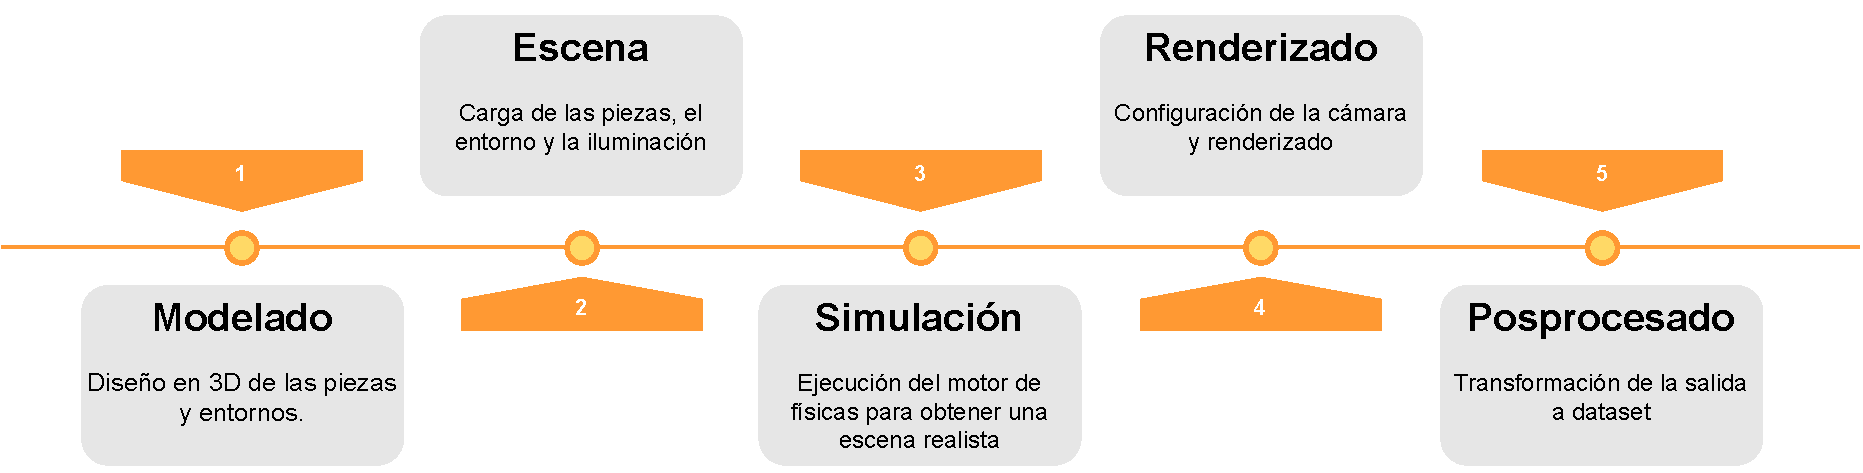
\includegraphics[width=0.9\textwidth]{Dataset/Arquitectura generador.pdf}
	\caption{Esquema de la arquitectura del sistema}
	\label{chap:Generación de un dataset fig:Arquitectura generador}
	\vspace{-5pt}
\end{figure}

Como se puede observar en la \autoref{chap:Generación de un dataset fig:Arquitectura generador}, se trata de un proceso iterativo constituido por varias etapas que se ejecutan en serie para la generación de cada nueva imagen. A excepción de la primera etapa que consiste en la generación de los modelos 3D, esta etapa no forma parte del generador pero este depende de la existencia de un modelo 3D con el que poder trabajar.

En esta etapa se han diseñado múltiples piezas de diferentes tamaños con la ayuda de Blender así como múltiples entornos sobre los que más adelante se dispondrán las piezas. Para las piezas se parte de un archivos .stl que contienen la información dimensional de las piezas. Estos han sido cargados en Blender donde se ha modificado el número de triángulos para mejorar el rendimiento y la suavidad de las piezas. Y se ha generado las texturas necesarias para las piezas las cuales incluyen defectos y patrones que deben de variar para cada instancia de estas añadiendo así aleatoriedad. Los entornos se han desarrollado por completo en Blender y se caracterizan por ser sencillos y planos. Su objetivo es contener a las piezas y no formar 0 confundirse con estas. Para los entornos se empleará una textura aleatoria para cada imagen de una librearía \textit{open source} CCTextures y constituida por más de mil seiscientas texturas de alta calidad.

Las piezas grandes requieren del uso de códigos QR que permitan en la etapa de posprocesado (\ref{chap:Generación de un dataset sec:Posprocesado}) extraer la información necesaria. Es por ello que en la etapa de modelado se debe de crear duplicados de las piezas grandes a los que se les insertará códigos QR en las zonas con posibles puntos de agarre.

Partiendo de los modelos y texturas necesarios, el sistema desarrollado puede empezar a generar imágenes:

\begin{enumerate}
\item Escena: Carga del entorno, de las piezas, la iluminación y la cámara
\begin{itemize}
\item Entorno: Se escoge de forma aleatoria uno de los entornos disponibles y se carga dentro de blender. A continuación, se escoge una de las texturas disponibles y se aplica en la totalidad del entorno. Por último, se centra el entorno y se deshabilita el cuerpo dentro del motor de físicas. De esta forma se fija la posición del entorno y este pasa a ser inalterable.

\item Piezas: Se escoge de forma aleatoria el número de piezas que estarán presentes en la escena (se establecen mínimos y máximos dependiendo del tamaño de la pieza) y se cargan dentro de blender. Por último, se define una propiedad \textit{category\_id} que más adelante será usada para identificar las distintas piezas.

\item Iluminación: Se parte de la base de que el entorno de trabajo real estará bien iluminado, por ello que se han definido unas condiciones de iluminación fijas y óptimas que permitan reducir las sombras. Se planteo emplear una iluminación aleatoria pero esta daba lugar a demasiadas sombras y dificultaba ver el contorno de las piezas oscuras.

\item Cámara: Para asemejarse a la realidad se ha fijado una cámara cenital a la escena y se ha implementado las parámetros intrínsecos de la cámara real que se va a emplear dentro de blender.
\end{itemize}

\item Simulación: activación de las piezas, posicionamiento de las piezas y simulación física.
\begin{itemize}
\item Activación de las piezas: se activa el motor de físicas para todas las piezas de forma que se vea afectadas por la gravedad y el entorno.
\item Posicionamiento de las piezas: con la ayuda de la \acs{api} de BlenderProc se posicionan todas las piezas de forma aleatoria dentro de un volumen de trabajo. El volumen de trabajo se fija en base a las dimensiones del entorno y la posición y orientación de la pieza se determina de forma aleatoria con el motor de aleatoriedad de numpy y BlenderProc.
\item Simulación física: se ejecuta una simulación física en la que se deja caer las piezas sobre el entorno/zona de trabajo. Se ejecuta el motor hasta que todas las piezas se vuelvan estáticas o se alcance el máximo tiempo de simulación de cuatro segundos.
\end{itemize}

\item Renderizado: configuración del motor de renderizado, renderizado y escritura de la salida de blender.
\begin{itemize}
\item Configuración: dependiendo del tamaño de la pieza se fija la configuración necesaria.
\begin{itemize}
\item Piezas grandes: resolución 3840x2160, 50 muestras y se activa el mapa de normales y de profundidad.
\item Piezas pequeñas: resolución 1920x1080, 25 muestras.
\end{itemize}
\item Renderizado: se activa el proceso o procesos de renderizado dependiendo del tamaño de la pieza.
\item Salida: se transfiere el resultado de los renderizados del archivo temporal de trabajo de blender al lugar de salida deseado.
\end{itemize}
\end{enumerate}

\begin{figure}[ht]
\centering
\begin{tabular}{cccc}
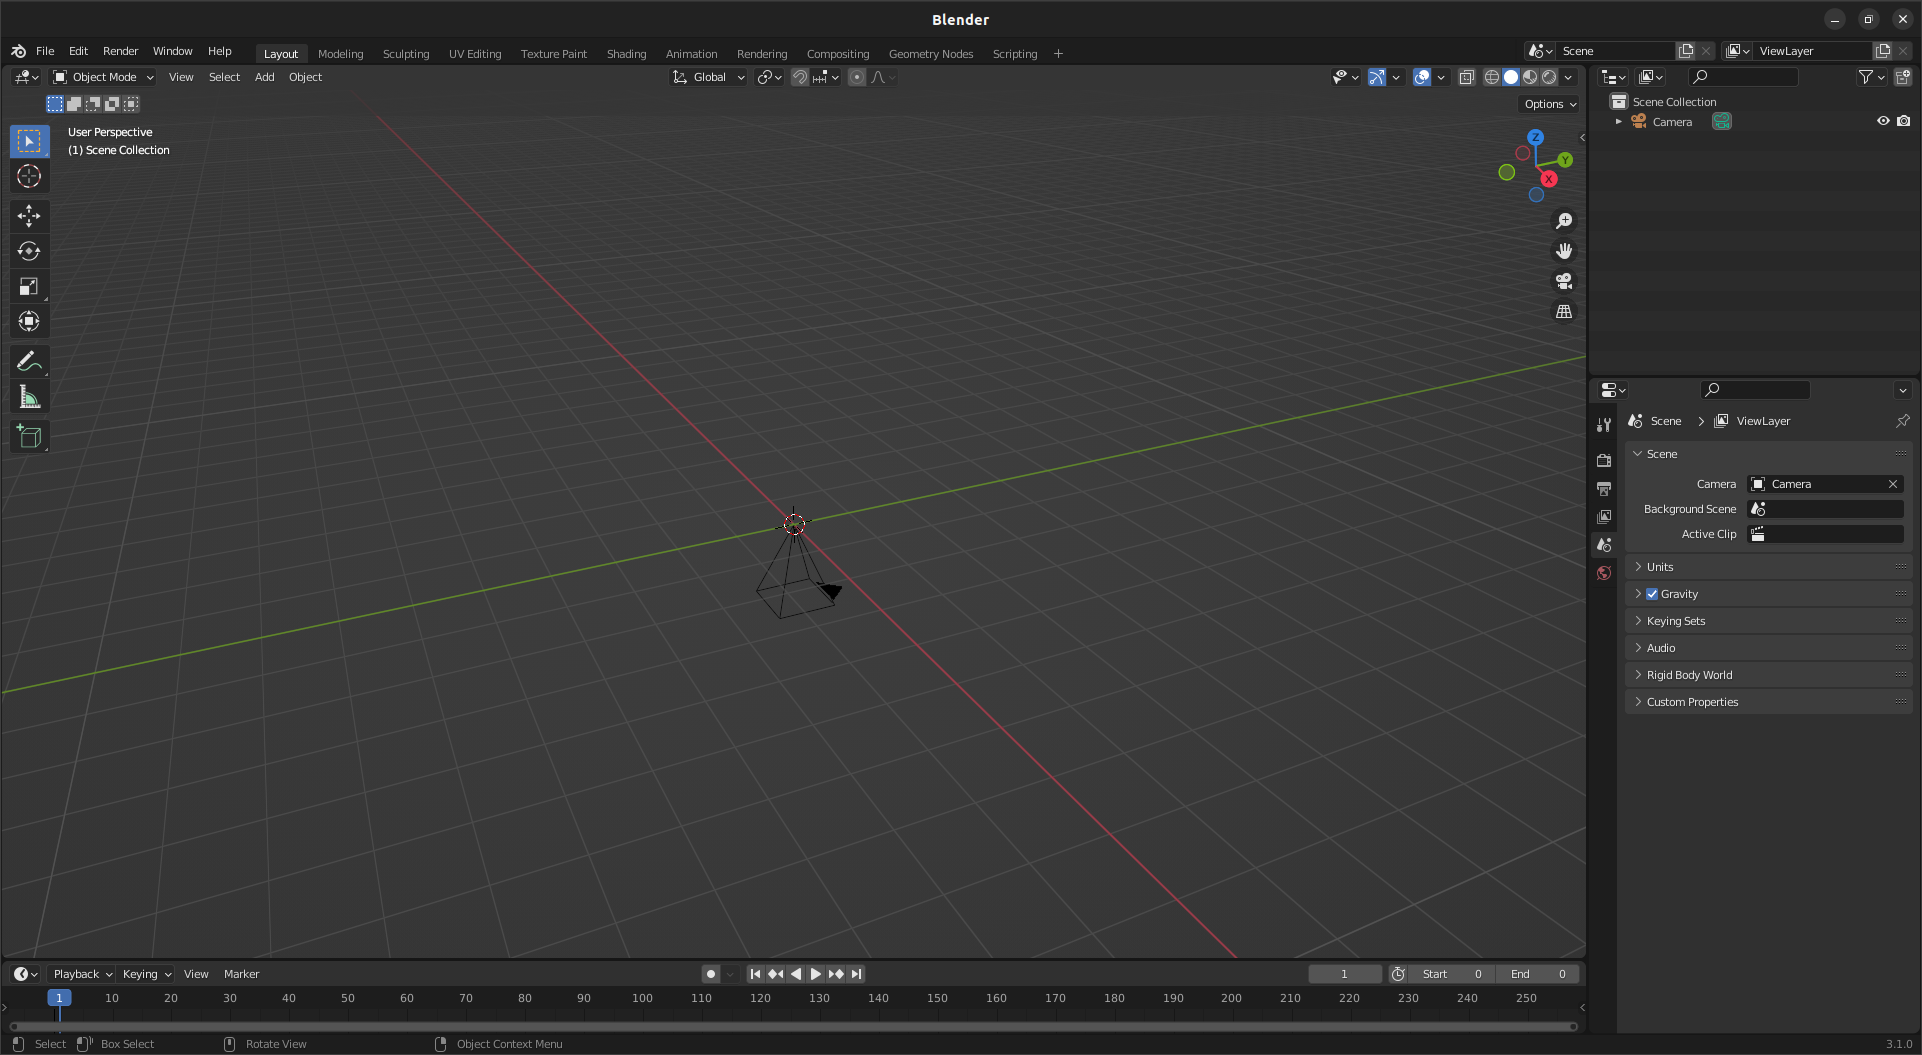
\includegraphics[width=0.3\textwidth]{Dataset/blender_normal_1.png} &
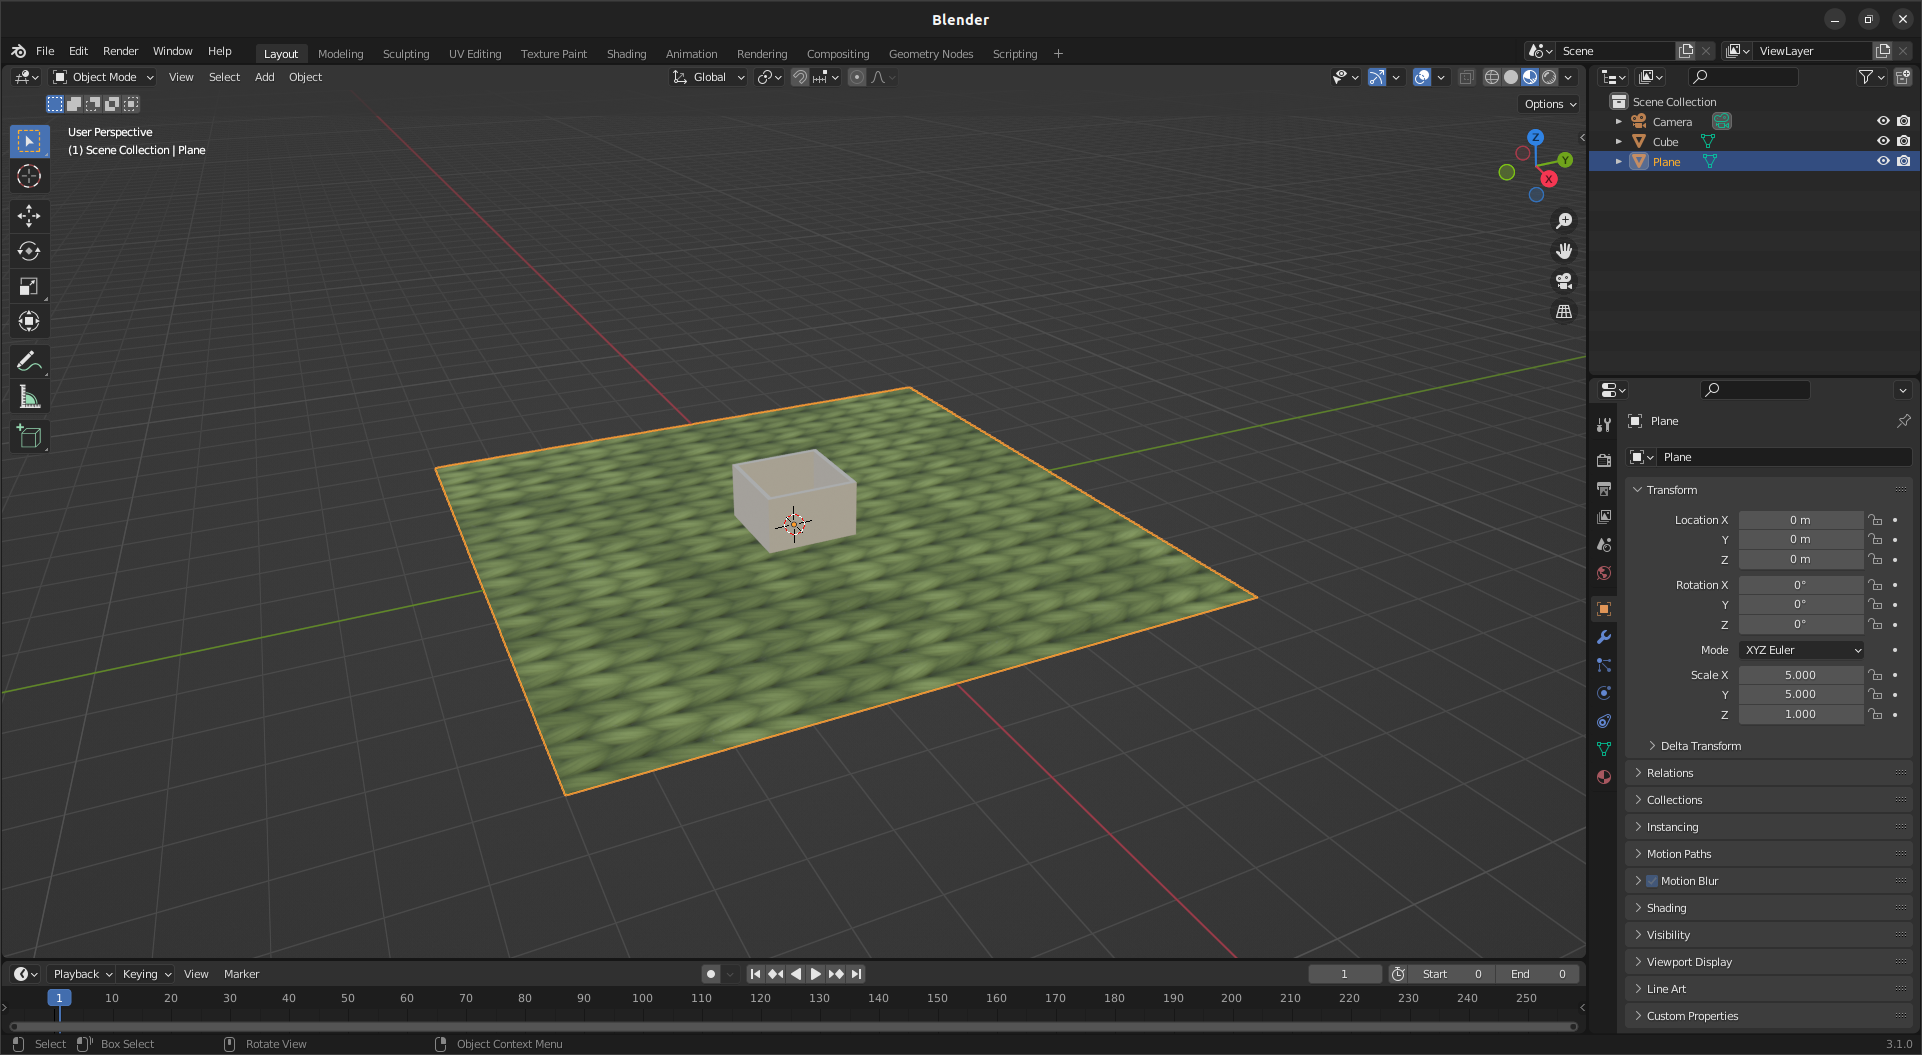
\includegraphics[width=0.3\textwidth]{Dataset/blender_normal_2.png} &
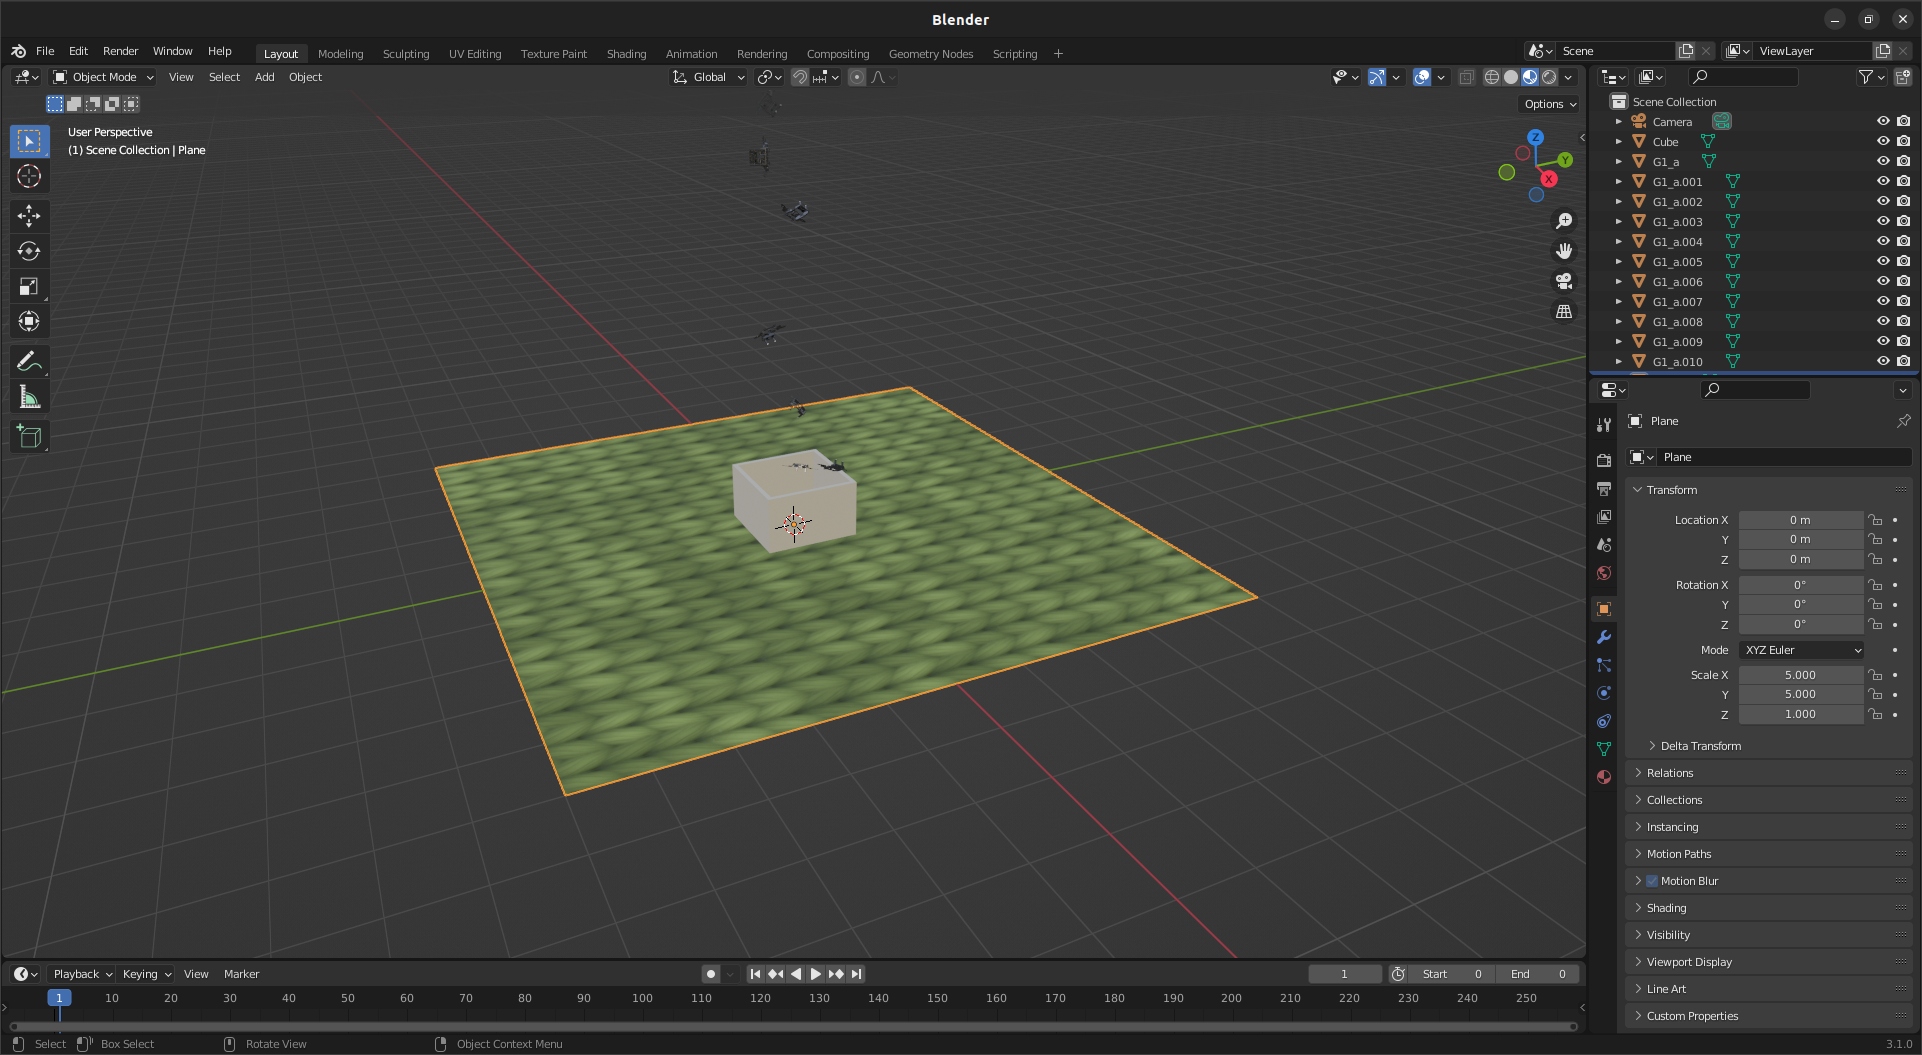
\includegraphics[width=0.3\textwidth]{Dataset/blender_normal_3.png} \\
Inicio  & Carga del escenario & Carga de piezas  \\[6pt]
\end{tabular}
\begin{tabular}{cccc}
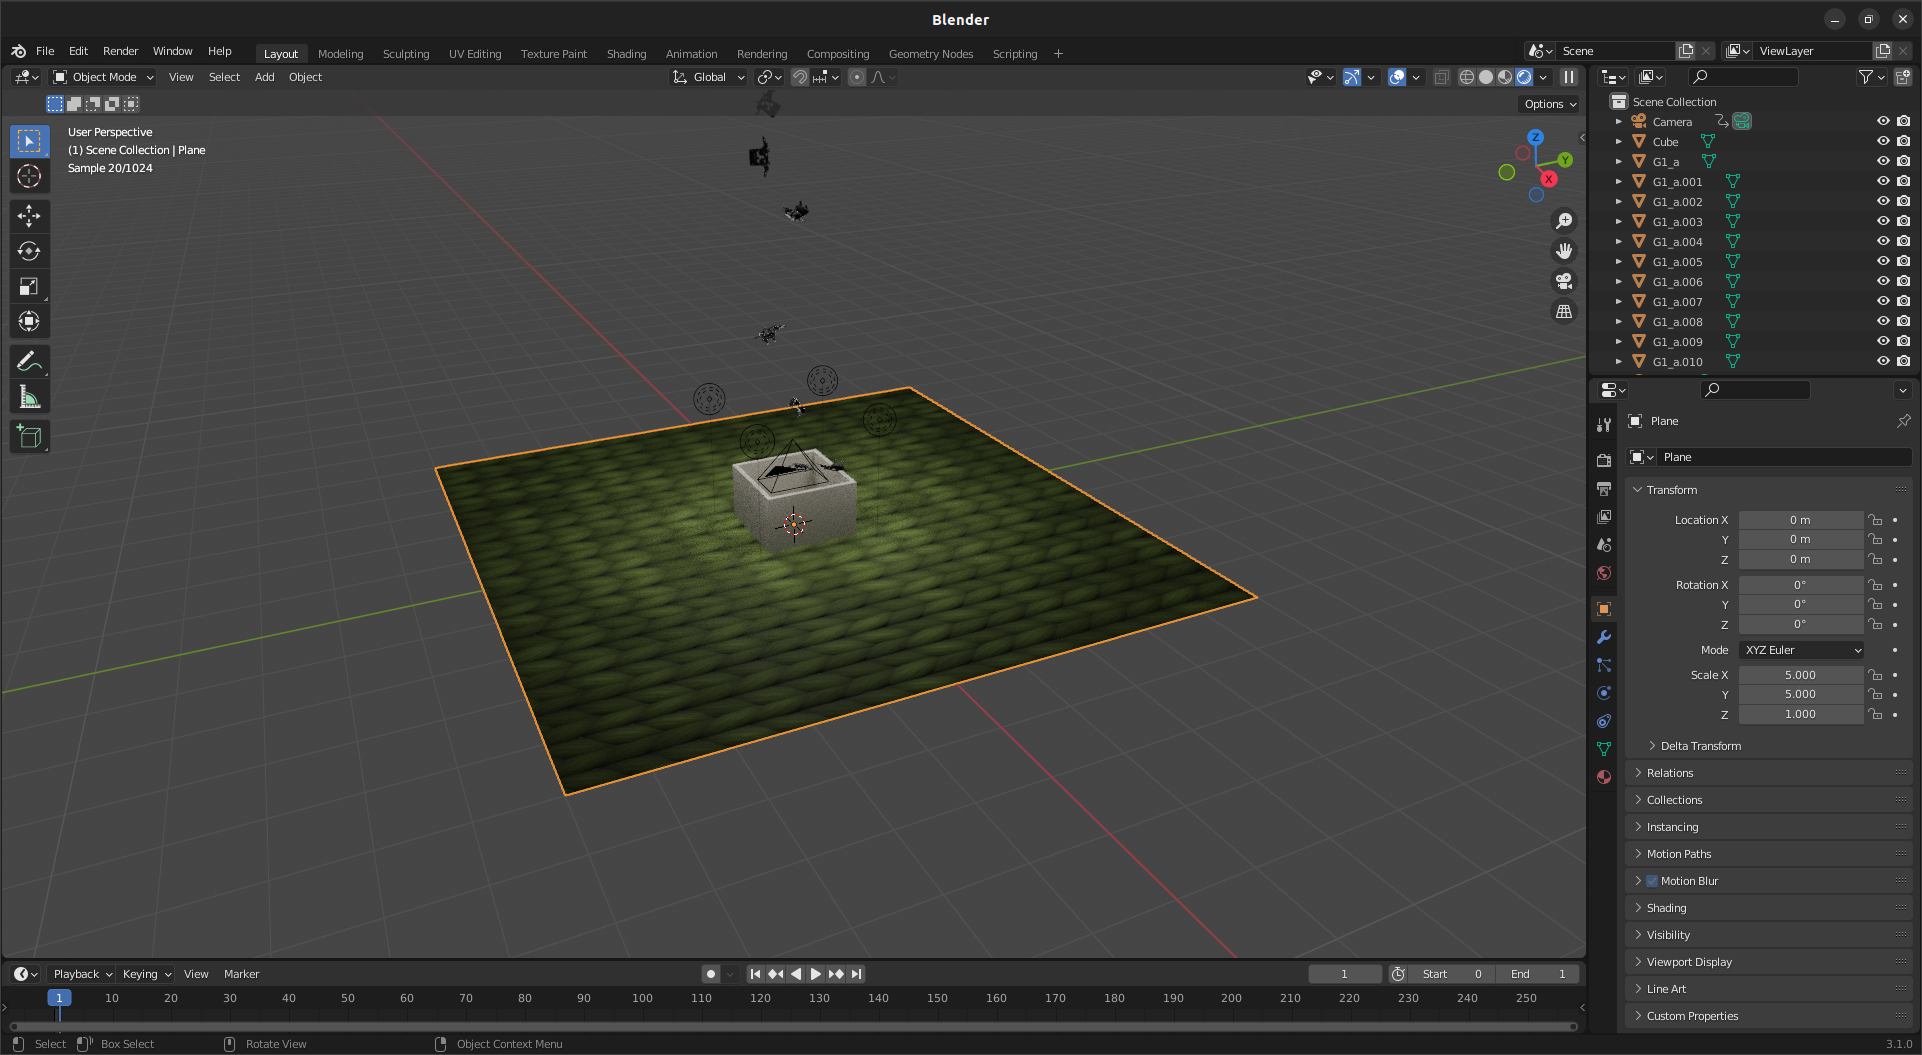
\includegraphics[width=0.3\textwidth]{Dataset/blender_normal_4.png} &
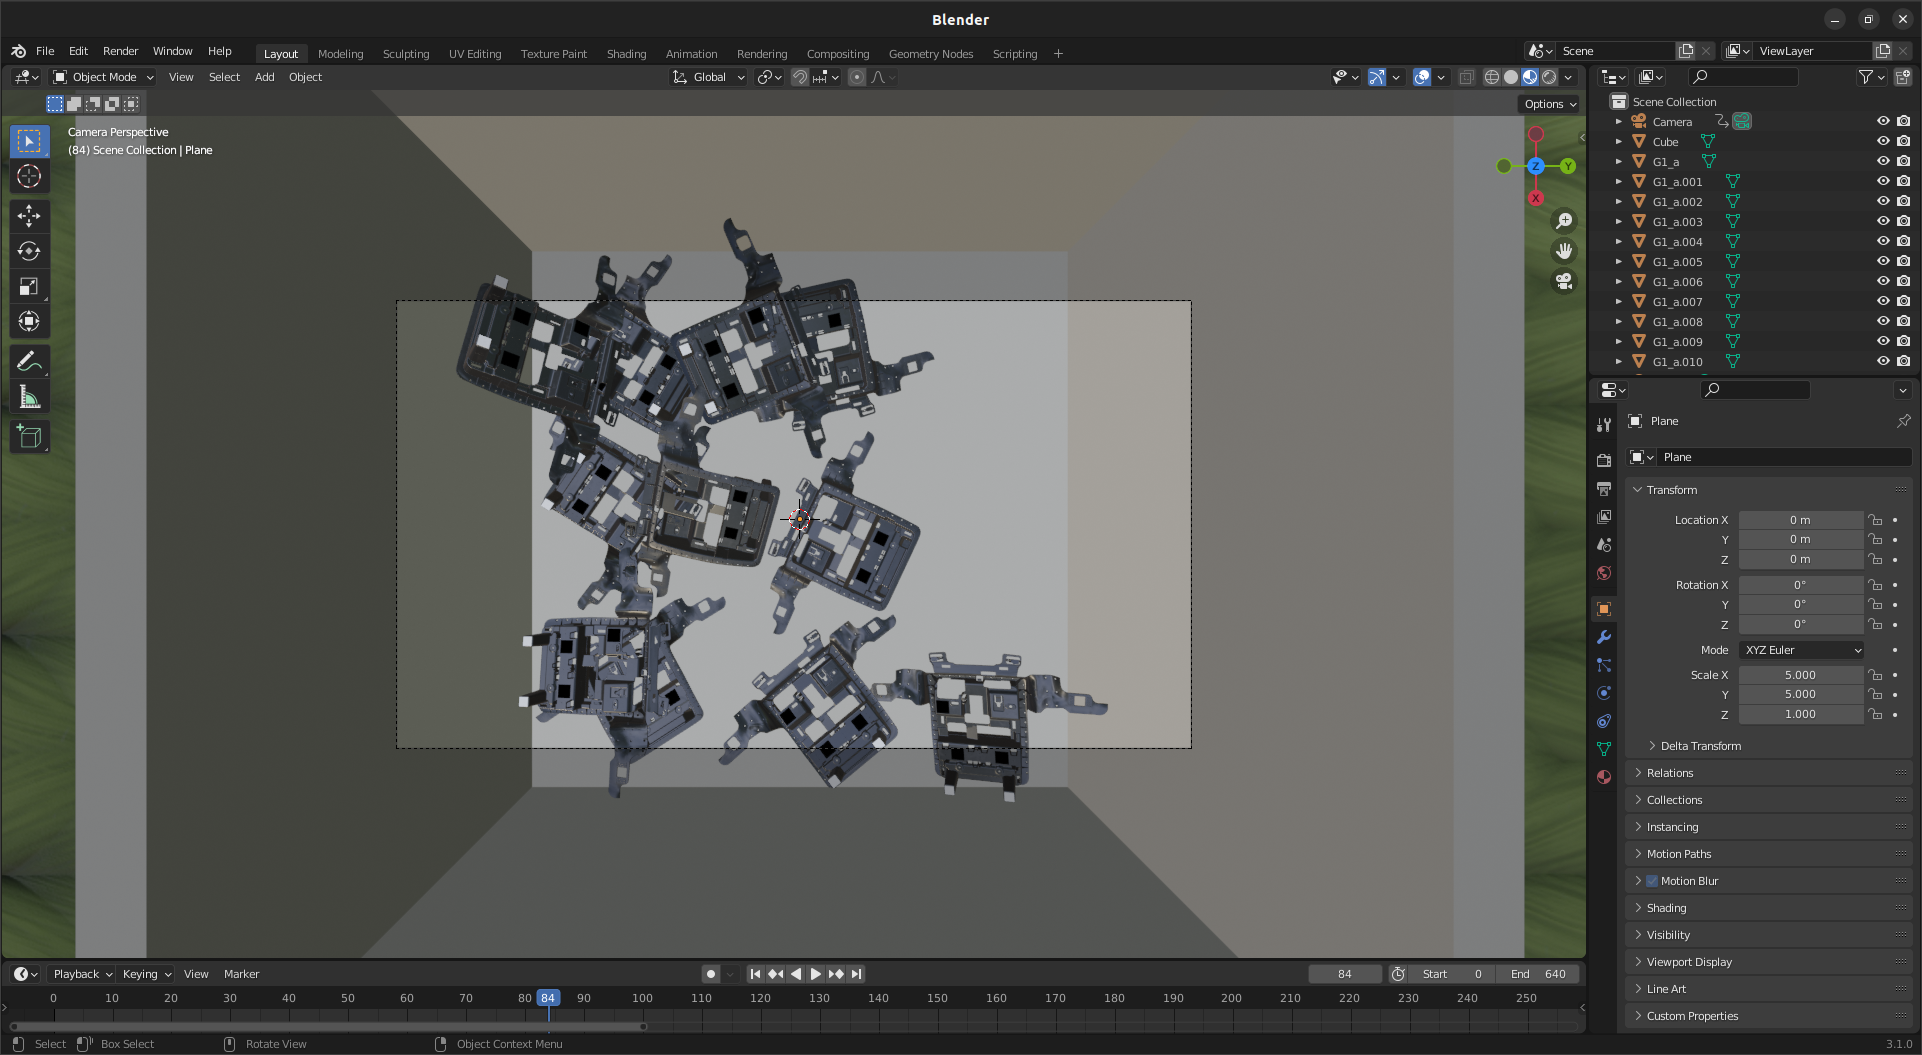
\includegraphics[width=0.3\textwidth]{Dataset/blender_normal_5.png} &
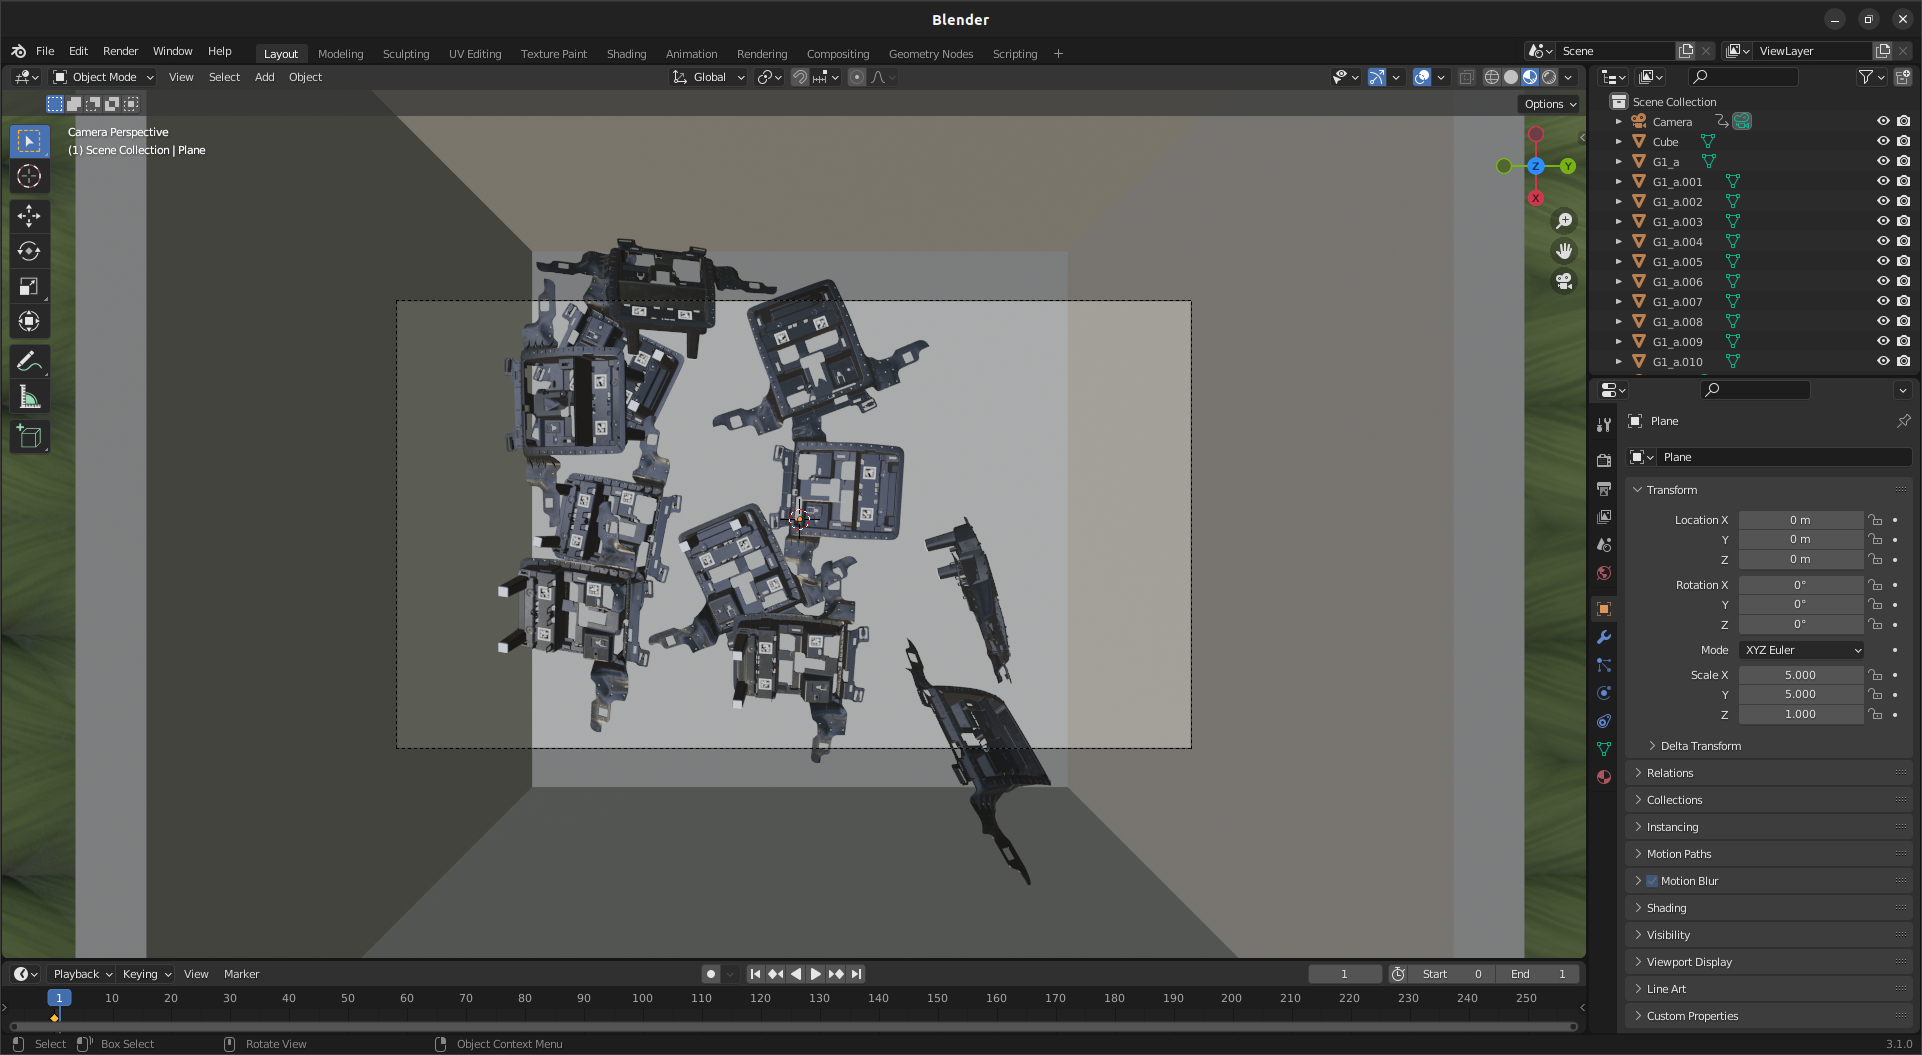
\includegraphics[width=0.3\textwidth]{Dataset/blender_aruco_1.png} \\
Iluminación y cámara  & Configuración normal & Configuración aruco  \\[6pt]
\end{tabular}
\begin{tabular}{cccc}
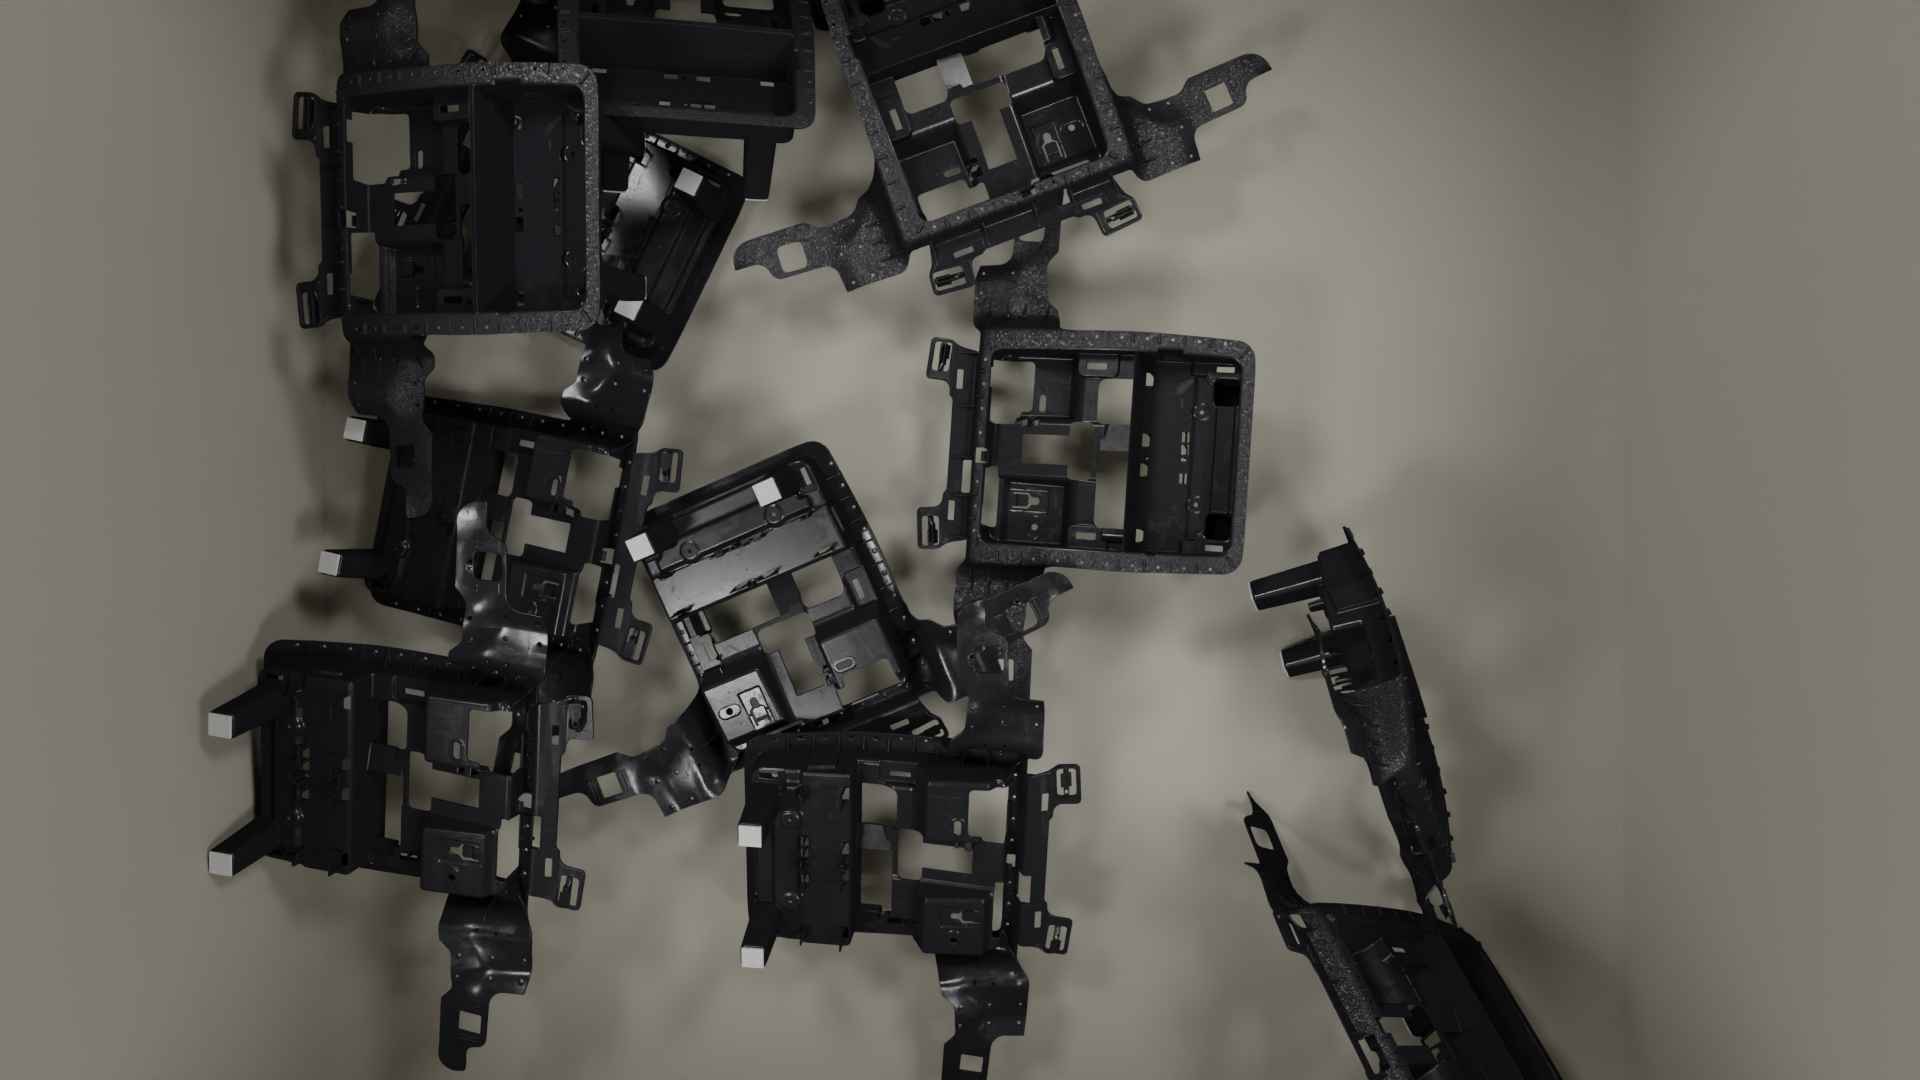
\includegraphics[width=0.3\textwidth]{Dataset/blender_normal_6.png} &
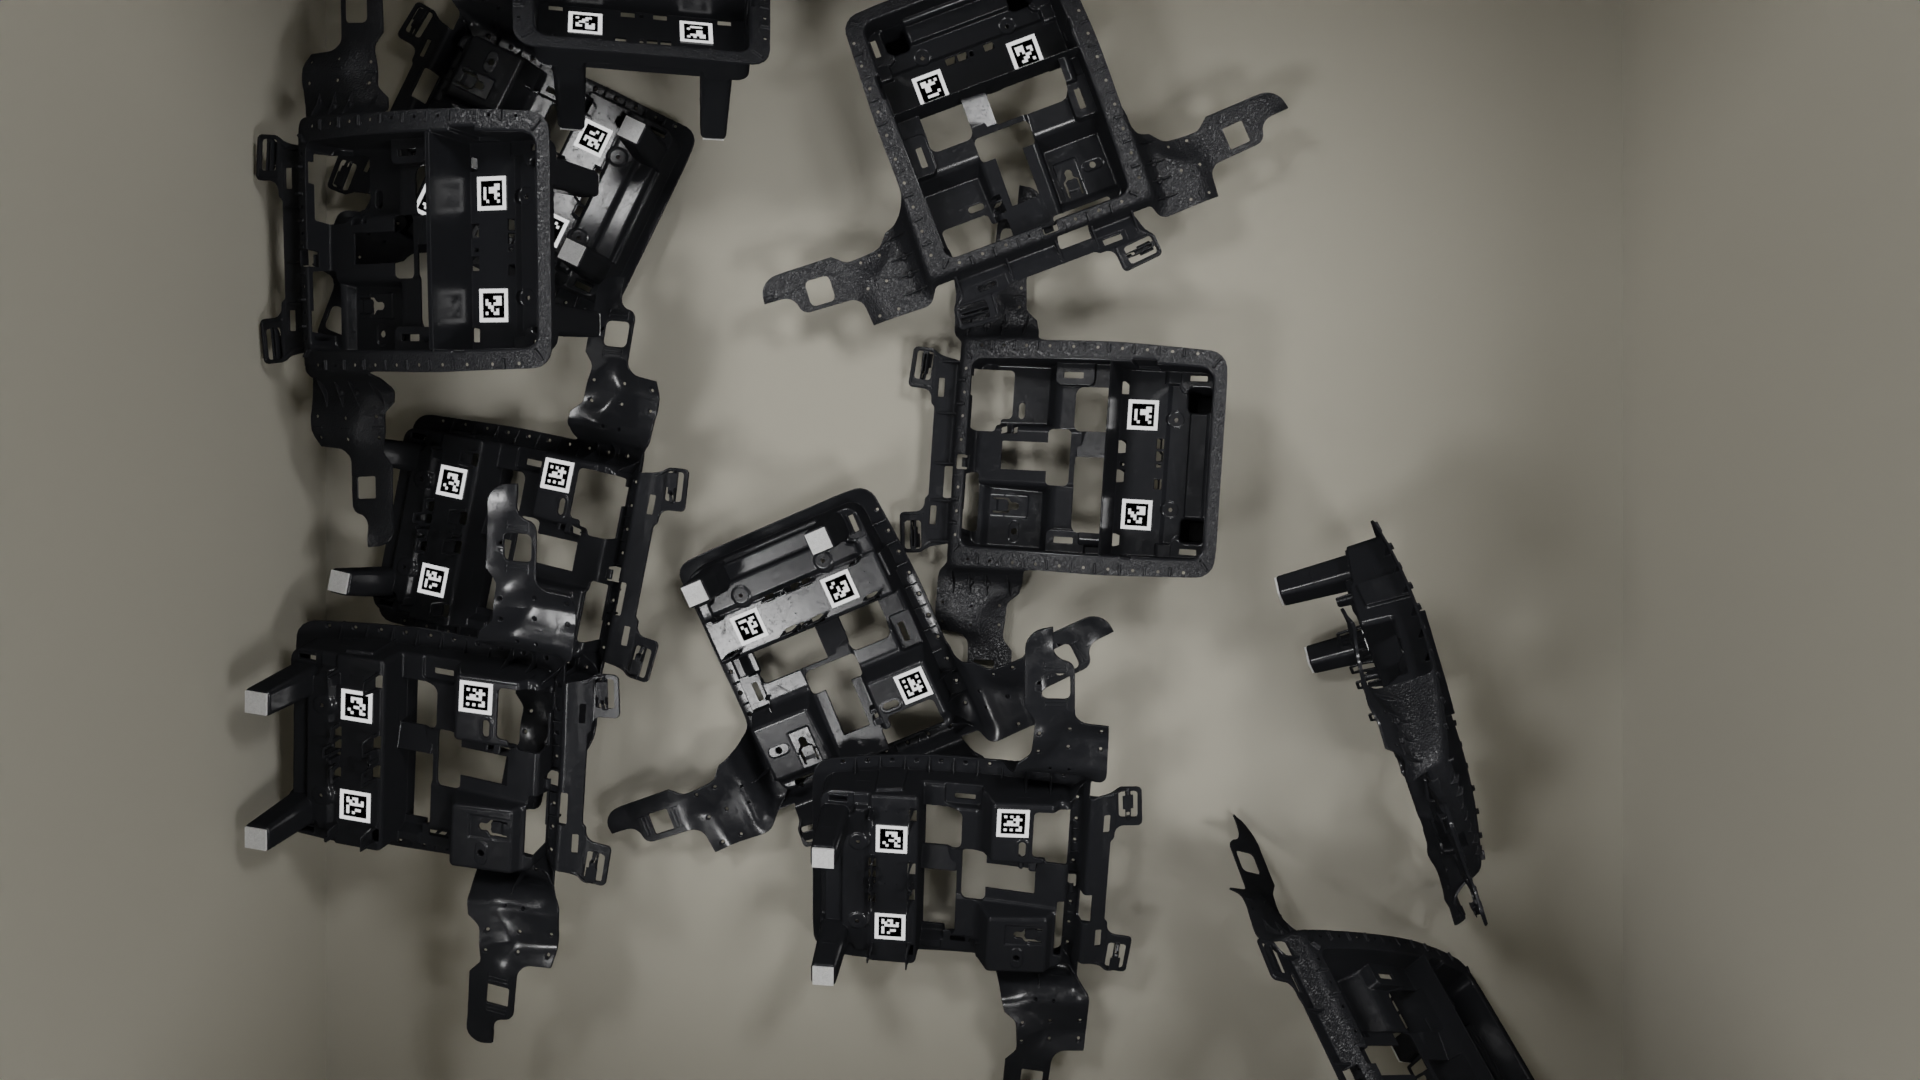
\includegraphics[width=0.3\textwidth]{Dataset/blender_aruco_2.png} \\
Render normal  & Render Aruco  \\[6pt]
\end{tabular}
\caption{Proceso de generación de imágenes}
\label{chap:Generación de un dataset fig:Proceso de generación}
\end{figure}


\section{Posprocesado}
\label{chap:Generación de un dataset sec:Posprocesado}
El \textit{dataset} deseado debe de contener para cada imagen una lista de todas las piezas presentes asi como su posición y los puntos de agarres disponibles. Esta información no se puede obtener de forma directo con Blender y BlenderProc, es por ello que se ha tenido que desarrollar varios sistemas de posprocesado específicos para cada uno de los componentes de la red neuronal.

\begin{itemize}
\item Posición (\textit{YOLO}): el primer procesado se caracteriza por ser una simple transformación de la información generada por Blender y BlenderProc a un formato que la red neuronal pueda entender. El generador de imágenes es capaz de crear un archivo de texto conteniendo la posición de las piezas en la imagen y el mapa de segmentación. Sin embargo, estas se encuentran en un formato distinto al empleado por la red neuronal. La transformación empleada consiste en un cambio de origen de la posición de las piezas y en la eliminación del resto de información que no es relevante. El proceso a seguir se muestra a continuación:
\vspace{5 mm}
\lstinputlisting[language=Python]{codigo/Prepare_Dataset_YOLO.py}
\vspace{5 mm}

\item Zonas de interés (\textit{Tiny YOLO}): el segundo procesado debe de determinar para cada piezas las posibles zonas de agarre. Para ello se debe de obtener para cada imagen un recorte de cada pieza presente en la imagen. Y la posición de las zonas de interés de cada recorte. Para llevar a cabo esta tarea se va a emplear la librearía Aruco que se caracteriza por poder detectar códigos QR con precisión, rapidez y eficiencia. El proceso a seguir se muestra a continuación:
\vspace{5 mm}
\lstinputlisting[language=Python]{codigo/Prepare_Dataset_TINY_YOLO.py}
\vspace{5 mm}

\item Vectores normales (Regresor): el objetivo es obtener los vectores normales y el punto de agarre para cada pieza. Por ello la salida en este caso será una imagen individual para cada pieza y un archivo de texto para cada punto de la pieza. En este archivo se almacenarán los centros de cada punto y las coordenadas de su vector normal. El proceso para la obtención de la imagen de cada pieza individual es idéntico al de las zonas de interés. Este posprocesado se caracteriza por el tratamiento de la imagen de normales y la generación de los archivos de texto con la información de cada punto de agarre. El proceso a seguir se muestra a continuación:
\vspace{5 mm}
\lstinputlisting[language=Python]{codigo/Prepare_Dataset_Regressor.py}
\vspace{5 mm}

\end{itemize}


\section{Aleatoriedad}
\label{chap:Generación de un dataset sec:Aleatoriedad}
Uno de los factores más importantes durante el desarrollo de este sistema es el sesgado. Se debe de evitar que el sistema genere un \textit{dataset} sesgado lo cual implica comprobar y asegurar la aleatoriedad de los resultados obtenidos. Para ello se empleará siempre que sea posible motores de aleatoriedad. Estos se caracterizan por ser capaces de obtener distribuciones uniformes (la mayor expresión de la aleatoriedad ya que todos los resultados son equitativamente probables). Con la excepción del generador de rotaciones aleatorias, ya que debido a la naturaleza de los ángulos de euler la distribución no puede ser uniforme. Durante el proceso de generación de imágenes se emplea un total de tres motores de aleatoriedad. Para asegurar la veracidad de estos tres motores, se ha realizado una serie de pruebas con diferentes semillas y múltiples muestras. A continuación, se muestras los resultados de todos los motores de aleatoriedad empleados.

El primer motor empleado se trata del generador de una distribución uniforme de numpy. Como su nombre indica, se encarga de generar un valor entre los máximos y mínimos establecidos de forma que todos los valores presenten la misma probabilidad. Este método es empleado para determinar el número de piezas que se deben de cargar así como su posición dentro de la zona de trabajo.

El segundo motor empleado es \textit{choice} del paquete \textit{random} de Python. Este se encarga de escoger de forma aleatoria un elemento de una lista. Se debe de asegurar de que todos los elementos presenten la misma probabilidad de ser escogidos. Este método es empleado para determinar que tipo de escenas, piezas y texturas se deben de emplear.

El último motor empleado es \textit{UniformSO3} de BlenderProc. Este se encarga de determinar una rotación aleatoria para las piezas. Esta rotación esta definida por ángulos de euler, es por ello que las distribuciones no deben de ser uniformes. Esto se debe a que una misma posición puede ser alcanzada por diferentes combinaciones de ángulos.

\begin{figure}[ht]
	\ContinuedFloat
	\centering
	\begin{subfigure}[b]{0.3\linewidth}
		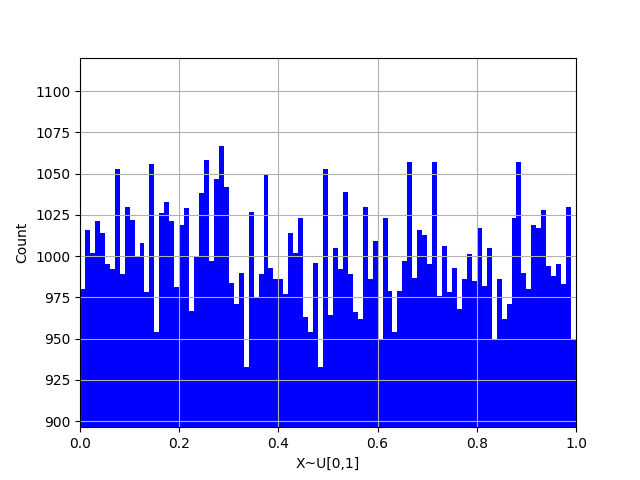
\includegraphics[width=\linewidth]{Dataset/numpy_uniform_histogram_10.png}
	\end{subfigure}
	\begin{subfigure}[b]{0.3\linewidth}
		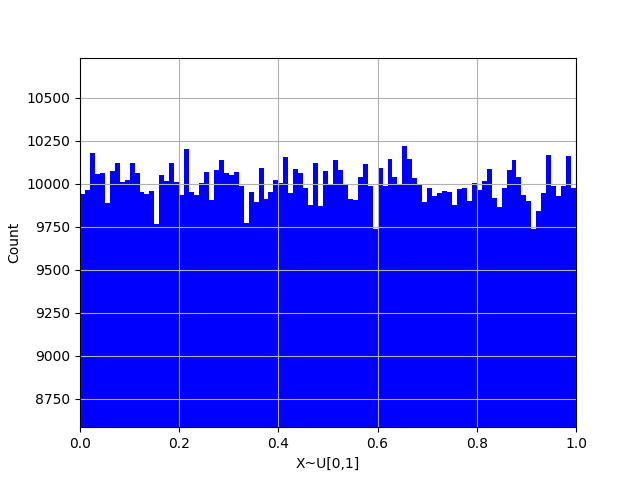
\includegraphics[width=\linewidth]{Dataset/numpy_uniform_histogram_100.png}
	\end{subfigure}
	\begin{subfigure}[b]{0.3\linewidth}
		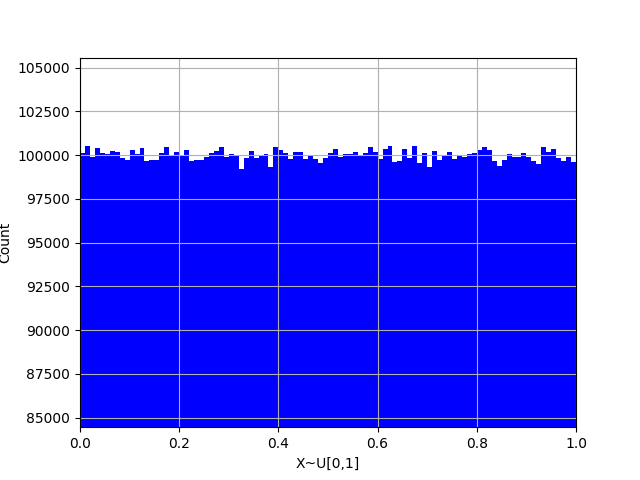
\includegraphics[width=\linewidth]{Dataset/numpy_uniform_histogram_1000.png}
	\end{subfigure}
	\caption{Aleatoriedad de una distribución uniforma generada por numpy}
	\label{chap:Generación de un dataset fig:numpy uniform}
	
	\begin{subfigure}[b]{0.3\linewidth}
		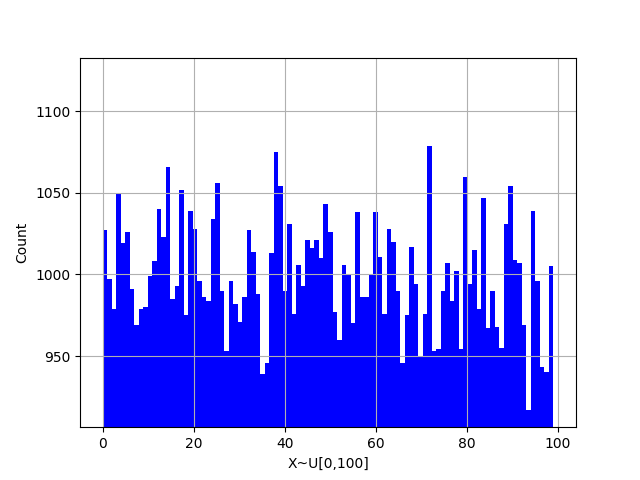
\includegraphics[width=\linewidth]{Dataset/random_choice_histogram_10.png}
	\end{subfigure}
	\begin{subfigure}[b]{0.3\linewidth}
		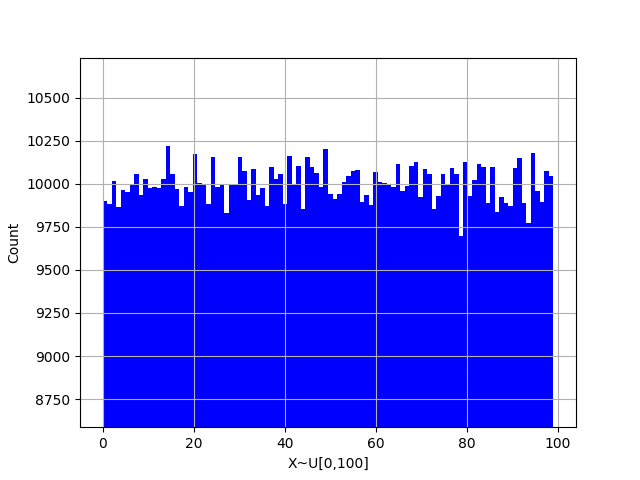
\includegraphics[width=\linewidth]{Dataset/random_choice_histogram_100.png}
	\end{subfigure}
	\begin{subfigure}[b]{0.3\linewidth}
		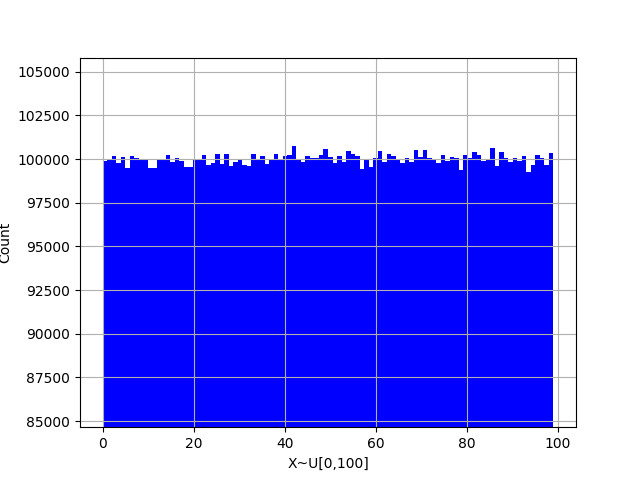
\includegraphics[width=\linewidth]{Dataset/random_choice_histogram_1000.png}
	\end{subfigure}
	\caption{Aleatoriedad del comando \textit{choice} del paquete \textit{random}}
	\label{chap:Generación de un dataset fig:random choice}
	
	\begin{subfigure}[b]{0.3\linewidth}
		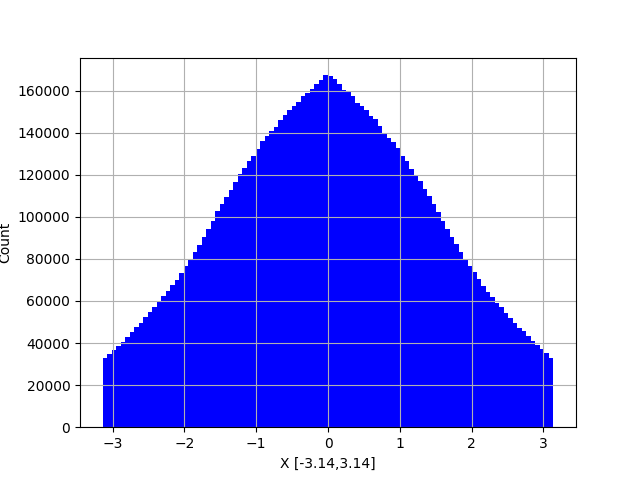
\includegraphics[width=\linewidth]{Dataset/blenderproc_uniformS03_histogram_1.png}
	\end{subfigure}
	\begin{subfigure}[b]{0.3\linewidth}
		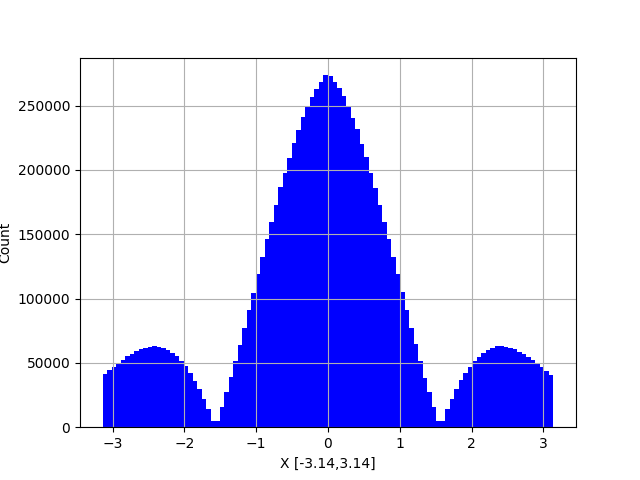
\includegraphics[width=\linewidth]{Dataset/blenderproc_uniformS03_histogram_2.png}
	\end{subfigure}
	\begin{subfigure}[b]{0.3\linewidth}
		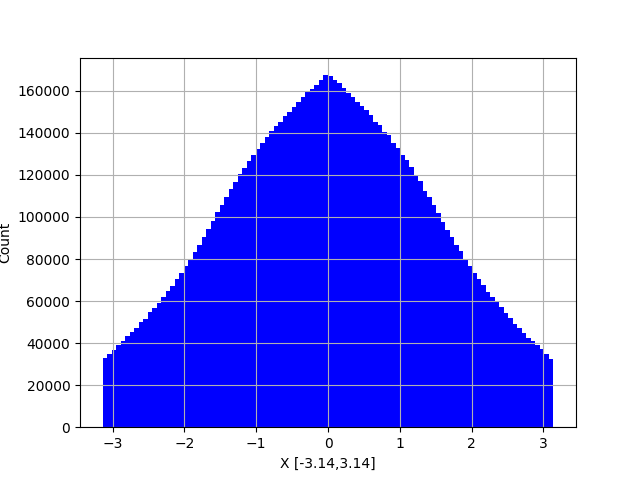
\includegraphics[width=\linewidth]{Dataset/blenderproc_uniformS03_histogram_3.png}
	\end{subfigure}
	\caption{Aleatoriedad de \textit{uniformSO3} del paquete BlenderProc}
	\label{chap:Generación de un dataset fig:uniformS03}
\end{figure}

\section{Resultados}
\label{chap:Generación de un dataset sec:Resultados}
Gracias a la implantación de un generador de imágenes se ha conseguido obtener un elevado número de instancias con las que poder entrenar la red neuronal que reflejan en gran medida la realidad. A continuación se muestran algunas de las imágenes obtenidas por es ambos sistemas.

\begin{figure}[ht]
	\ContinuedFloat
	\centering
	\begin{subfigure}[b]{0.3\linewidth}
		\includegraphics[width=\linewidth]{Dataset/Muestra_G1_a_sintetica.png}
	\end{subfigure}
	\begin{subfigure}[b]{0.3\linewidth}
		\includegraphics[width=\linewidth]{Dataset/Muestra_G3_sintetica.png}
	\end{subfigure}
	\begin{subfigure}[b]{0.3\linewidth}
		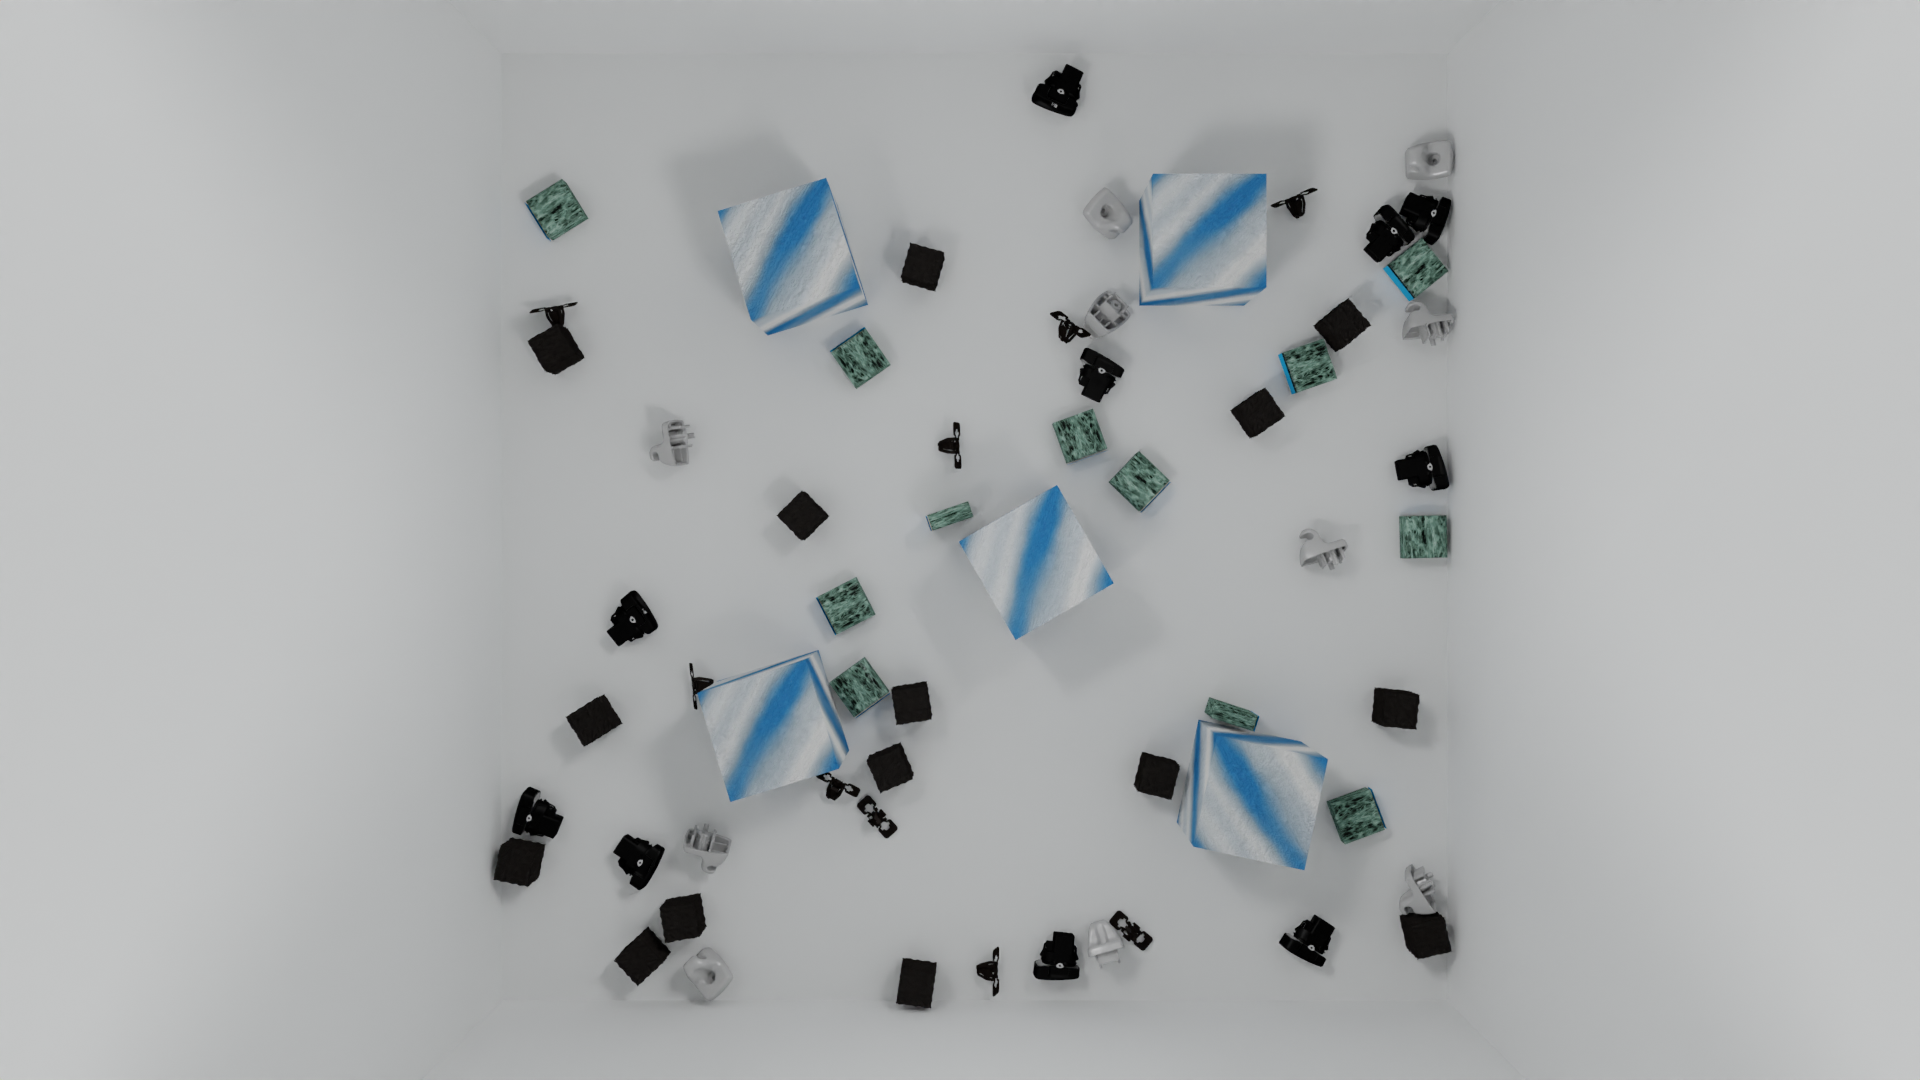
\includegraphics[width=\linewidth]{Dataset/Muestra_small_sintetica.png}
	\end{subfigure}
	\caption{Muestra de imágenes obtenidas mediante el generador de imágenes}
	\label{chap:Generación de un dataset fig:Muestras BlenderProc}

\end{figure}

Como se ha mencionado previamente, es importante entrenar modelos de redes neuronales con \textit{datasets} no sesgados. Esto implica que antes de entrenar un modelo se debe de analizar los datos para comprobar que se cumplen dichos requisitos. Para ello se han desarrollado una serie de \textit{scripts} en Python que permitirán mostrar el verdadero estado del \textit{dataset}.

Como para el desarrollo de este proyecto se deben de desarrollar tres modelos de redes neuronales, se debe de analizar los datos necesarios correspondiente a cada uno de estos modelos:

\begin{itemize}
\item \textit{YOLO}: se trata de la primera red neuronal empleada y desarrollada. Se encargará de detectar las piezas dentro de la zona de trabajo y se empleará como base para decidir que pieza se debe de recolectar. La salida de este modelo debe de ser las piezas presentes en la imagen y su posición. Por ello, para poder ser entrenada correctamente se debe de disponer de un número de instancias similares para cada pieza que se desea detectar.

\item \textit{Tiny YOLO}: una red neuronal menor y menos potente pero con una mayor especialización. Esta red se encargará de determinar regiones con posibles puntos de agarre dentro de las piezas (previamente identificadas por \textit{YOLO}). Esta segunda capa es especifica para cada pieza y solo se aplicará a aquellas piezas de elevado volumen. Es por ello que para el análisis de los datos de entrenamiento nos debemos de fijar de forma individual e independiente en cada pieza. En este caso nos vamos a centrar en las piezas G1 y G3 y en el número de instancias de cada zona de interés presente en estas.

\item Regresor: se trata de la última capa del sistema de visión artificial. Se basa en la salida del \textit{Tiny YOLO} y determina para cada una de las posibles regiones de interés el punto de agarre óptimo y su vector normal. Esta última capa es especifica para cada pieza y solo se aplicará a aquellas piezas de elevado volumen. Es por ello que para el análisis de los datos de entrenamiento nos debemos de fijar de forma individual e independiente en cada pieza. Además, al tratarse de un regresor es importante fijarse en la distribución de muestras con el fin de evitar emplear un \textit{dataset} sesgado. En este caso nos vamos a centrar en la pieza G1\_a.
\end{itemize}

\begin{figure}[ht]
	\ContinuedFloat
	\centering
	\begin{subfigure}[b]{0.9\linewidth}
		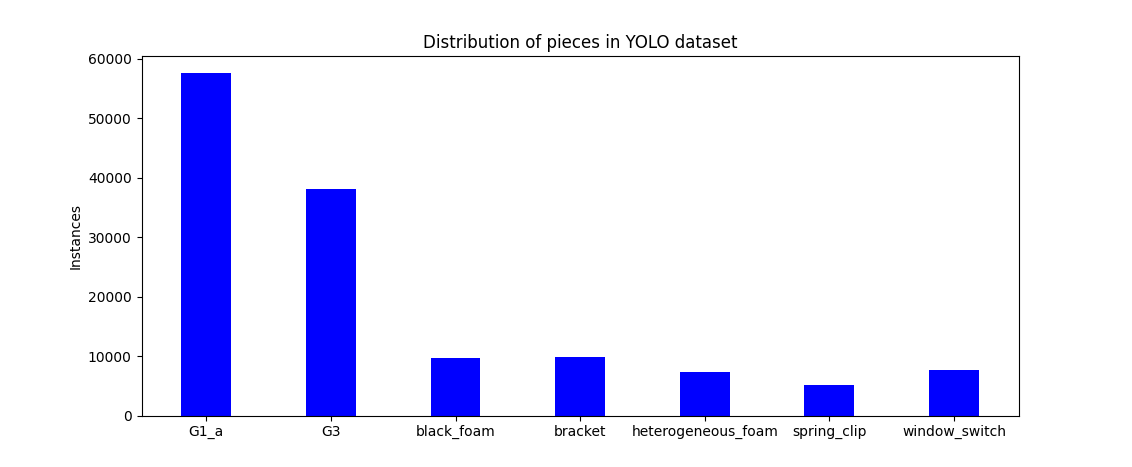
\includegraphics[width=\linewidth]{Dataset/instances_yolo.png}
	\end{subfigure}
	\caption{Instancias de cada pieza empleadas para entrenar el modelo basado en YOLO}
	\label{chap:Generación de un dataset fig:Instancias YOLO}
	
	\begin{subfigure}[b]{0.4\linewidth}
		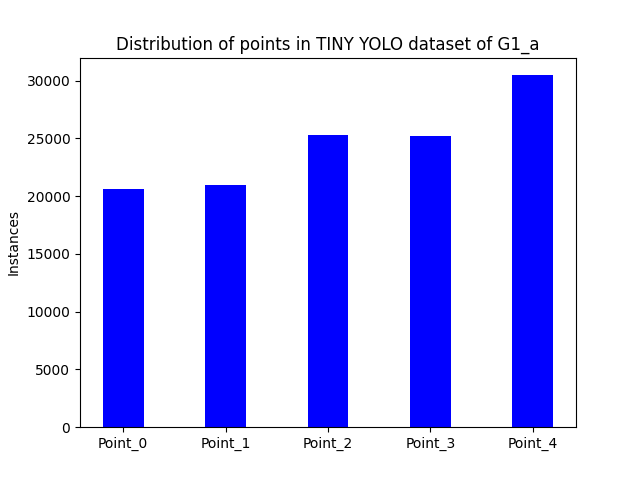
\includegraphics[width=\linewidth]{Dataset/instances_tiny_yolo_G1_a.png}
	\end{subfigure}
	\begin{subfigure}[b]{0.4\linewidth}
		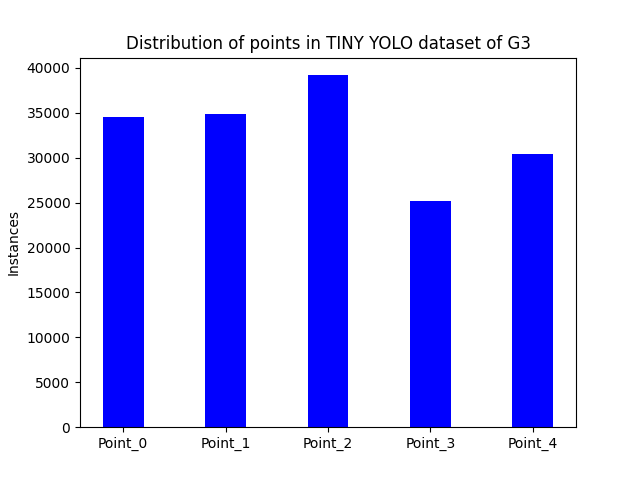
\includegraphics[width=\linewidth]{Dataset/instances_tiny_yolo_G3.png}
	\end{subfigure}
	\caption{Instancias de cada zona de interes empleadas para entrenar el modelo basado en Tiny YOLO}
	\label{chap:Generación de un dataset fig:Instancias Tiny YOLO}
	
	\begin{subfigure}[b]{0.9\linewidth}
		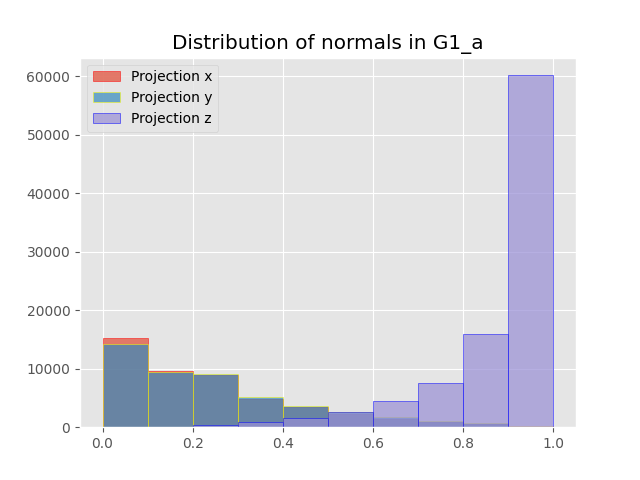
\includegraphics[width=\linewidth]{Dataset/normal_vector_projection_G1_a.png}
	\end{subfigure}
	\caption{Distribución de las proyecciones normales de los puntos de agarre de G1}
	\label{chap:Generación de un dataset fig:Sesgo G1}

\end{figure}


\section{Conclusiones y futuros desarrollos}
Gracias a los resultados mostrados en el capitulo anterior se puede observar el verdadero potencial del generador de imágenes, pero también se aprecia los fallos y puntos de mejora. El sistema ha demostrado ser una opción viable capaz de representar la realidad de forma fiel. Capaz de mantener una constante aleatoriedad a la vez que asegura la replicación. Y ha demostrado ser un sistema adaptable y escalable capaz de trabajar con cualquier tipo de pieza.

Pero a su vez ha mostrado varios fallos de diseño que se deben a error humano y no del sistema. Desgraciadamente el \textit{dataset} generado no es perfecto ya que presenta un elevado sesgo a pesar de representar en gran medida la realidad. A la hora de desarrollar el sistema se enfoco el proyecto en recrear la realidad en lugar de pensar en que tipo de \textit{dataset} se requiere para entrenar la red neuronal. Y debido a la naturaleza de las piezas la realidad es un escenario sesgado en donde la mayoría de las piezas se encuentran en una posición horizontal.

Para evitar este problema en futuros desarrollos se recomienda la introducción de nuevos escenarios con diferentes geometrías que permitan obtener instancias de las piezas con mayor riqueza y en diferentes posiciones. Este tipo de escenarios no deben de presentar un suelo plano sino que deberán de presentar diferentes elevaciones de forma que al apoyarse las piezas no queden en posición horizontal.
